\documentclass[14]{article}
\usepackage{graphicx} % Required for inserting images
\usepackage{amsmath}
\usepackage{amssymb}
\usepackage{enumitem}
\usepackage{multicol}
\usepackage{hyperref}
\usepackage{tikz}
\usepackage{geometry}
\geometry{
a4paper,
total={170mm,257mm},
left=20mm,
top=20mm,
bottom=20mm
}
\usepackage{titling}
\graphicspath{{./images/}}
\renewcommand\maketitlehooka{\null\mbox{}\vfill}
\renewcommand\maketitlehookd{\vfill\null}
\title{COMP2521: Data Structure and Algorithms}
\author{Haeohreum Kim (z5480978)}
\date{2023 T3}

\begin{document}
\begin{titlingpage}
\maketitle
\tableofcontents
\end{titlingpage}
\newpage
\section{Sorting algorithms}
Sorting algorithms are a fundamental problem in computer science. At the core, having a sorted list of some objects lets us
do very useful things to it - specifically within COMP2521, we see binary search being used often to achieve $O(\log n)$ performance. \\ 
Visualisations of ecah of these algorithms can be found at \href{https://visualgo.net/en/sorting}{VisuAlgo}.
\subsection{Comparison sorts}
Quadratic algorithms are often very easy to implement - but also come at a time cost. Quadratic algorithms generally have 
nested loops, which are easy to understand, as it compares each node with every single other node n times. \\ 
$\mathbf{O(n^2) \text{ \textbf{algorithms}}}$
\begin{enumerate}
	\item Selection Sort \\ 
	Selection sort works by creating a sorted component and an un-sorted component. The sort works by finding the smallest
	element left in the unsorted component, and then inserting it in the appropiate place in the sorted component. \\ 
	Worst case time complexity: $O(n^2)$ \\ 
	Best case time complexity: $O(n^2)$ \\ 
	Stable: No \\ 
	\item Insertion Sort \\ 
	Insertion sort is similar to selection sort, but instead, just chooses the next element to insert into the 
	sorted component. It begins (usually) with the left most element being considered 'sorted'. \\ 
	Worst case time complexity: $O(n^2)$ \\ 
	Best case time complexity: $O(n)$ \\
	Stable: Yes \\ 
	\item Bubble Sort \\
	Bubble sort works in a cyclical manner, where it iterates through the array, compares adjacent elements,
	and swaps them if they are out of order. \\ 
	Worst case time complexity: $O(n^2)$ \\ 
	Best case time complexity: $O(n)$ \\
	Stables: Yes \\ 
\end{enumerate}
$\mathbf{O(nlogn) \text{\textbf{ algorithms}}}$ \\ 
$O(n\log n)$ sorts are more difficult to implement, but offer superior, noticeable performance in large datasets.
\begin{enumerate}
	\item Quicksort \\ 
	Quicksort is a divide and conquer algorithm, which works by choosing a \emph{pivot}, and then partitoning
	the elements into sets that are smaller than the element, and bigger than the element. Notably, quicksort 
	can have a worst-case time complexity of $O(n^2)$, when an array is sorted. There are multiple different 'pivot' choices
	that a programmer can make, begin:
	\begin{enumerate}
		\item Naive \\ 
		Naive quick sort chooses the first element (or last, or some fixed element) as the pivot. 
		This is the easiest to implement, but also, the worst performing. 
		\item Median-of-three \\ 
		Median-of-three quick sort chooses the median of the first, middle and last element as the pivot.
		This minimises the risk of choosing a worst case pivot, but doesn't entirely remove it. The worst case
		is still $O(n^2)$, but the average time complexity will be better empirically.
		\item Randomised \\ 
		Randomised quick sort chooses a random pivot. This has the best empirical performance. It is highly
		unlikely that the worst choice may be chosen.
	\end{enumerate}
	Worst case time complexity: $O(n^2)$ \\ 
	Best case time complexity: $O(nlogn)$ \\ 
	Stable: No 
\item Merge Sort \\
	Merge Sort is also a divide and conquer algorithm, which works by splitting the array into two halves, and then
	recursively sorting the two halves, and then merging them together. Merge sort is a stable algorithm, and is
	often used in practice. \\ 
	Worst case time complexity: $O(nlogn)$ \\ 
	Best case time complexity: $O(nlogn)$ \\ 
	Stable: Yes  
\end{enumerate}
\subsection{Non-comparison sorts}
Non-comparison sorts don't compare elements directly - but rather use some sort of external sorting method. \\
\textbf{Radix sort} \\ 
Radix sort is a non-comparison sort, which works by sorting the elements by their individual digits. 
It works by sorting the elements into "buckets" by their least significant digit, and then moving onto the next digit.
This is repeated until the most significant digit is reached. (From the last digit to the first digit).
An example of radix sort would be:  
\section{Binary search trees}
A binary search tree is a tree with nodes with at most two children, and has the property that the left child is less than the parent.
With this, a search can be performed in $O(\log n)$ time.
\subsection{Traversal}
There are three main types of traversal: 
\begin{enumerate}
	\item Pre-order traversal \\
	Pre-order traversal can be seen as "stay left" algorithm. It works by visting the current node, and then recursively 
	going down the tree, marking the nodes. The pre-order traversal can be represented as:
	\begin{verbatim}
print(node)
preorder(node.left)
preorder(node.right)
	\end{verbatim}
	\item In-order traversal \\
	In-order traversal can be seen as the "left parent right" algorithm - starting from the bottom left, and sweeping upwards,
	making sure each node is visited. In a BST, it would go bottom left, it's parent, it's right sibling, 
	the parent's parent, and then the parent's sibling subtree.
	\begin{verbatim}
inorder(node.left)
print(node)
inorder(node.right)
	\end{verbatim}
	\item Post-order traversal \\
	Post-order traversal can be seen as the "left right parent" algorithm. It trys to stay as low as possible within the tree,
	but then sweeps up similar to an in-order traversal. In a BST, it would go bottom left, it's sibling, THEN it's parent,
	then the parent's sibling subtree, and then the parent's parent.
	\begin{verbatim}
postorder(node.left)
print(node)
postorder(node.right)
	\end{verbatim}
\end{enumerate}
\pagebreak
\subsection{Balanced BST's and AVL Trees}
\subsubsection{Calculating balance}
The size balance of a tree, is calculated by the formula:
\begin{center}
    $size(left) - size(right)$
\end{center}
The height balance of a tree is calculated by the height of the left subtree, minus the height of the right subtree.
It is calculated by:
\begin{center}
    $height(left) - height(right)$
\end{center}
This \emph{balance factor} should be calculated at each node, so that the tree gets balanced from the bottom up.
\begin{center}
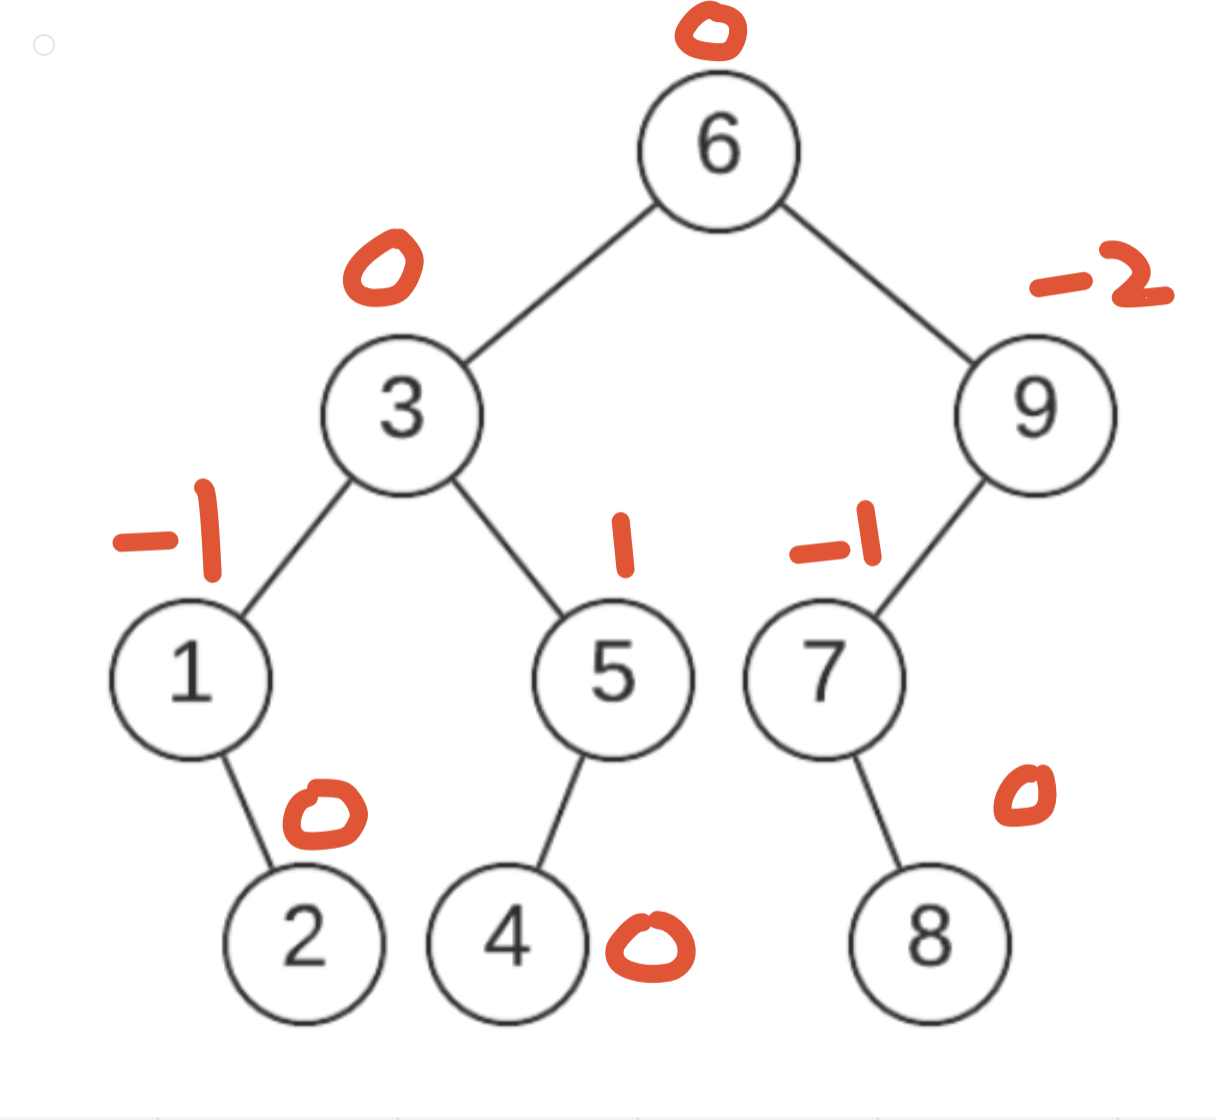
\includegraphics[scale=0.25]{images/balance_1.png}
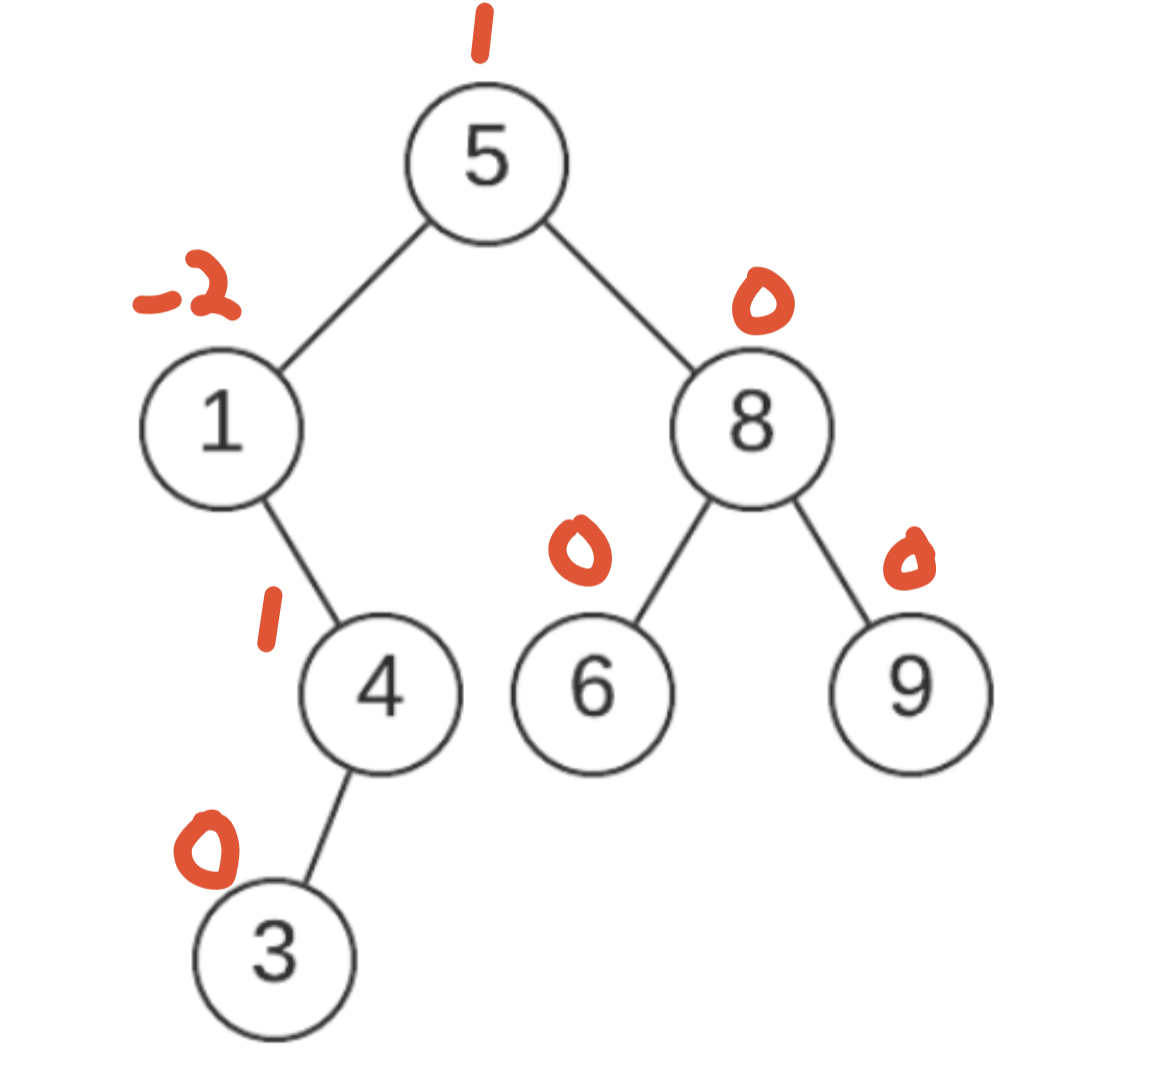
\includegraphics[scale=0.25]{images/balance_2.png}
\end{center}
\subsubsection{Rotations}
Rotations keep things balanced. If a tree is unbalanced $<-1$, then it requires a right rotation.
If a tree is unbalanced $>1$, then it requires a left rotation.
\begin{itemize}
	\item In different scenarios, you will need a left-right, right-right, right-left, and left-left rotation.
	\item Right-right and left-left rotations deal with degenerate cases, where the tree is unbalanced in one direction.
	\item Right-left and left-right rotations deal with the tree being unbalanced in two directions, in a zig-zag pattern.
\end{itemize}
\begin{center}
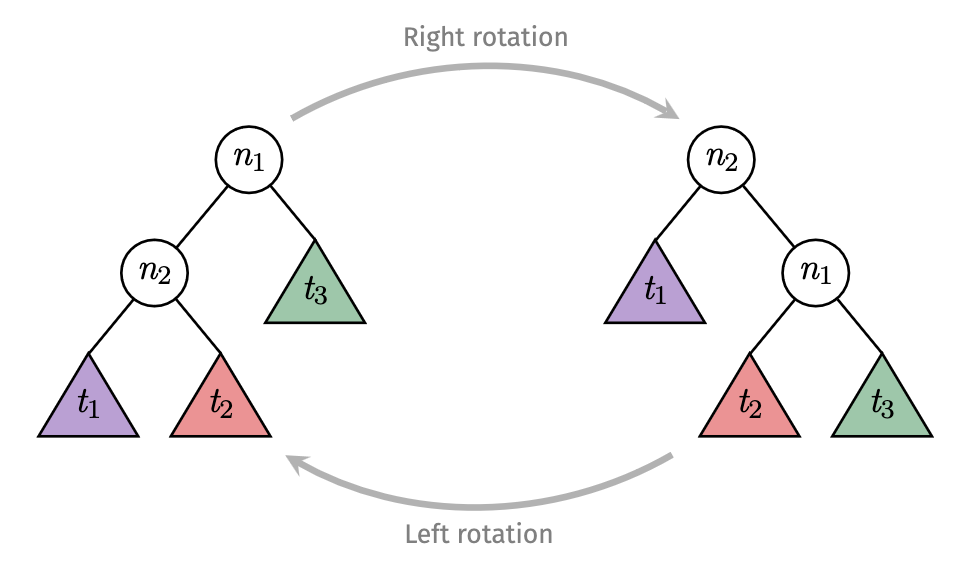
\includegraphics[scale=0.75]{images/rotations.png}
\end{center}
\pagebreak
\subsubsection{AVL Trees}
AVL trees are constructed by inserting nodes into a BST, and then rotating the tree if it becomes unbalanced.
This improves our worst time complexity to $O(\log n)$, as the tree is always balanced. \\ 
The steps are: 
\begin{enumerate}
	\item Insert the node into the tree, as you would normally.
	\item Calculate the balance factor of the node.
	\item If the balance factor is $<-1$ or $>1$, then rotate the tree.
		\begin{enumerate}
			\item If the balance factor is $<-1$ and the value of the inserting node is less 
			than the rotating node's left child, then perform a right-right rotation.
			Else, perform a right-left rotation.
			\item If the balance factor is $>1$ and the value of the inserting node is greater
			than the rotating node's right child, then perform a left-left rotation.
			Else, perform a left-right rotation.

		\end{enumerate}
	\item Repeat until the tree is balanced.
\end{enumerate}

\subsubsection{Global Rebalancing}
Global rebalancing works by partitioning the tree into subtrees, and the rebuilding and rebalancing the entire tree
as a whole. This is opposed to what an AVL tree does, which is \emph{local rebalancing}, which only rebalances the tree
at the node it is inserted at. Global rebalancing ensures a perfect balance.
\begin{verbatim}
rebalance(tree)
    t = partition(t, size(t) / 2)
    t.left = rebalance(t.left)
    t.right = rebalance(t.right)
\end{verbatim}
\subsubsection{Root Insertion}
Root insertion is a technique used to insert a new node into the BST, and then make it the root node. \\
Root insertion works as such:
\begin{verbatim}
insert(tree, value)
    if tree empty 
        value <- tree
    else if value < tree->item
        insert(tree.left, value)
        tree = rotateRight(tree)
    else if value > tree->item
        insert(tree.right, value)
        tree = rotateLeft(tree)

    return tree
\end{verbatim}
\subsubsection{Randomised Insertion}
Due to the way AVL trees work, a sorted or partially sorted array of data will result in a worst case performance.
This is due to the amount of rotating that is required. Random insertion randomly chooses an element from the to-insert 
set, and then inserts this into the AVL tree, minimising the risk of having to rebalance a degenerate tree.
\pagebreak
\section{Graphs}
Graphs are a data structure that are used to represent relationships between objects. They are made up of vertices and edges.
With the possibility of far more than 2 "children" (now called, adjacent vertices), graphs are very powerful, and also
contain more complex algorithms.  
\subsection{Terminology}
\subsubsection{Sparseness}
For a simple graph, it will always be true such that:
\begin{center}
    $|E| \leq \frac{|V|(|V| - 1)}{2}$
\end{center}
if $|E|$ is closer to $|V|^2$, then the graph is \emph{dense}. If $|E|$ is closer to $|V|$, then the graph is \emph{sparse}.
\subsubsection{Vertices, edges, and the connections between them}
\begin{itemize}
    \item Two vertices are \emph{adjacent} if there is an edge between them.  
    \item The \emph{degree} of a vertex is the number of edges that are incident to it. 
    \item An edge is incident to two adjacent vertices if the edge connects them.
    \item A \emph{path} is a sequence of vertices, where each consecutive pair are adjacent.
    \item A \emph{simple path} is a path where no vertices are repeated.
    \item A \emph{cycle} is a path, where the first and last vertices are the same.
    \item A \emph{complete graph} is a graph where every vertex is adjacent to every other vertex.
    \item A \emph{subgraph} is a graph that is a subset of another graph.
    \item A \emph{clique} is a complete subgraph.
\end{itemize}
\subsection{Representations}
We can represent graphs in multiple ways, each with their own advantages and disadvantages. 
This will depend on the scenario, and what we want to do with the graph.
\subsubsection{Array of Edges}
An array of edges is a simple way to represent a graph. It is a list of edges, where each edge is a tuple of two vertices. \\ 
Its properties are (in general):
\begin{itemize}
    \item Space complexity: $O(|E|)$
    \item Time complexity: 
        \begin{itemize}
            \item Finding if two vertices are adjacent: $O(|E|)$
            \item Finding all adjacent vertices: $O(|E|)$
            \item Inserting an edge: $O(|E|)$
            \item Deleting an edge: $O(|E|)$
            \item DFS/BFS: $O(|E|^2)$
        \end{itemize}
\end{itemize}
\subsubsection{Adjacency Matrix}
An adjacency matrix is a matrix of size $|V| \times |V|$, where each cell represents whether the two vertices are adjacent.
Its properties are (in general):
\begin{itemize}
    \item Space complexity: $O(|V|^2)$
    \item Time complexity: 
        \begin{itemize}
            \item Finding if two vertices are adjacent: $O(1)$
            \item Finding all adjacent vertices: $O(|V|)$
            \item Inserting an edge: $O(1)$
            \item Deleting an edge: $O(1)$
            \item DFS/BFS: $O(|V|^2)$
        \end{itemize}
\end{itemize}
\subsubsection{Adjacency List}
An adjacency list is a list of lists, where each list represents the adjacent vertices of a vertex. \\ 
Its properties are (in general):
\begin{itemize}
    \item Space complexity: $O(|V| + |E|)$
    \item Time complexity: 
        \begin{itemize}
            \item Finding if two vertices are adjacent: $O(|V|)$
            \item Finding all adjacent vertices: $O(|V|)$
            \item Inserting an edge: $O(|V|)$
            \item Deleting an edge: $O(|V|)$
            \item DFS/BFS: $O(|V| + |E|)$
        \end{itemize}
\end{itemize}
\section{Traversal}
\subsection{Breadth First Search}
Visits all adjacent vertices of a vertex, then adds the neighbours of such adjacent verticies. Generally implemented
iteratively with a Queue.
\subsection{Depth First Search}
Visits an adjacent vertex of a vertex, adds the adjacent vertex's neighbours, and goes "deep". Generally implemented 
with a stack iteratively, or can also be done recursively.
\section{Graph problems}
\subsection{Cycle checking}
Seeing if a cycle exists is useful for certain problems, such as finding a minimum spanning tree.
\begin{enumerate}
    \item Perform a DFS, starting from any vertex.
    \item If at any point, a vertex has already been visited, then there exists a cycle.
\end{enumerate}
\begin{verbatim}
dfsHasCycle(G, v, visited):
visited[v] = true 
for each neighbour w of v:
    if visited[w] = true:
        return true
    else if dfsHasCycle(G, w, visited):
        return true
\end{verbatim}
\pagebreak
\subsection{Connected components}
A connected component is a maximally connected subgraph.
\begin{center}
    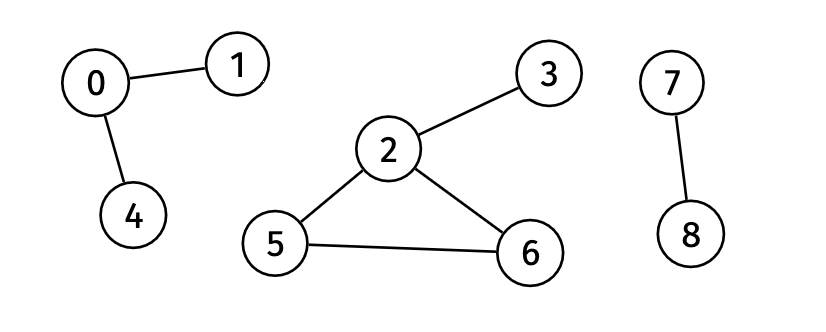
\includegraphics[scale=0.75]{images/con_comps.png}
\end{center}
\begin{enumerate}
    \item Choose a vertex, and perform a DFS starting at that vertex. Assign all vertices
        visited to component 0. 
    \item After the initial DFS, if any vertex has not been assigned a component,
        perform a DFS on that vertex. During this DFS, assign all vertices visited to
        the component 1
    \item Repeat until all vertices have been assigned a component.
\end{enumerate}
\begin{verbatim}
dfsComponents(G, v, visited, componentOf, compNo):
    componentOf[v] = compNo
    for each neighbour w of v in G:
        if componentOf[w] = -1:
            dfsComponents(G, w, componentOf, compNo)
\end{verbatim}
\subsection{Hamiltonian Path/Circuit}
Combinatorial problem $O(n!)$, so very big time cost. A hamiltionian path is a path that visits every vertex exactly once.
A hamiltionian circuit is a hamiltionian path that ends at the starting vertex.
\begin{enumerate}
    \item Use DFS to check every single possible paths
    \item Keep track of the number of vertices left to visit
    \item If that number is 0, stop, and return true.
\end{enumerate}
\subsection{Euler Path/Circuit}
An Euler path/circuit problem is a polynomial-time problem. An Euler path is a path that visits every edge exactly once.
An Euler circuit is an Euler path that ends at the starting vertex.
\begin{enumerate}
    \item A graph has an Euler path iff exactly zero or two vertices have odd degree, and all verticies with non-zero degree
        belong to the same connected component.
    \item A graph has an Euler circuit iff every vertex has an even degree, and all verticies with non-zero degree belong 
        to the same connected component. 
\end{enumerate}
\subsection{Reachability}
Finding out if you can reach one vertex from another vertex is an important problem. For example, if I wanted to know if I can
visit Strathfield from Epping, I'd have to use a reachability algorithm. 
\subsubsection{Warshall's Algorithm}
Warshall's algorithm uses a reachability matrix to build up the problem from a single vertex. 
\begin{verbatim}
warshall(A):
    initialise neighbours prior

    for each vertex i in G
        for each vertex j in G
            for each vertex k in G:
                if tc[j][i] and tc[i][k]:
                    tc[j][k] = true
\end{verbatim}
\subsection{Shortest path}
Finding the shortest path from one vertex to another is a fundamental problem - and is heavily used throughout the real world.
An obvious example could be in Google Maps, where they use Djikstra's and A* (an extension of Djikstra's).
\subsubsection{Djikstra's Algorithm}
\begin{enumerate}
    \item Initialise predecessor and distance array. 
    \item Create a priority queue of the vertexes, with the distance as the priority.
    \item Remove a vertex, and explore v - for each edge v-w, check if a new shortest distance has been found.
    \item If so, update w's distance and predecessor.
\end{enumerate}
\subsection{Minimum spanning trees}
A minimum spanning tree is a subgraph of a graph, that is a tree, and connects all vertices together, with the minimum
possible weight.
\subsubsection{Prim's Algorithm}
\begin{enumerate}
    \item Start from any vertex, and add it to the MST.
    \item Chose the cheapest edge s-t such that:
        \begin{itemize}
            \item s has been added to the MST
            \item t has not been added to the MST
        \end{itemize}
    \item Repeat previous step until $|V| - 1$ edges have been added.
\end{enumerate}
\subsubsection{Kruskal's Algorithm}
\begin{enumerate}
    \item Add edges into a priority queue, sorted by weight.
    \item Choose the smallest edge, and add it to the MST.
    \item If the edge creates a cycle, remove the edge.
    \item Continue until there are $|V| - 1$ edges in the MST.
\end{enumerate}
\section{Hash Tables}
A hash tables are a data structure that maps keys to values. It is on average $O(1)$ for insertion, deletion and lookup.
\subsection{Hashing}
There are multiple different ways to hash; the objective is to be as random as possible. For strings, a simple hash could be
\begin{verbatim}
int hash(char *key, int N) {
    int sum = 0;
    for (int i = 0; key[i] != '\0'; i++) {
        sum += key[i];
    }
    return sum % N;
}
\end{verbatim}
\subsection{Collision resolution}
However, hashing isn't perfect. Over a dataset, collisions can occur. There are three different ways to deal with collisions, 
which have their own advantages and disadvantages.  \\ 
An important number is the \textbf{load factor} ($\alpha$) calculated by:
\begin{center}
    $\alpha = \dfrac{\text{number of items}}{\text{size of hash table}}$
\end{center}
\subsubsection{Seperate chaining}
Each array element in the hashmap is the head of a linked list. When a collision occurs, the new element is added to the linked list.
\subsubsection{Linear probing}
When a collision occurs, the new element is added to the next available slot in the array. This is done by incrementing the index.
If the hash of an element does not lead to the target element, the function will "linearly probe" the hashmap until it
finds the specific elemnt. 
\subsubsection{Double hashing}  
When a collision occurs, apply an alternate hash to it. This is done by incrementing the index by the alternate hash, until a
free spot is found. This improves our best time complexity of a collision search to $O(1)$.
\end{document}
